\documentclass{article}

\usepackage{polski}
\usepackage[margin=1in]{geometry}
\usepackage[parfill]{parskip}
\usepackage{amsmath}
\usepackage{graphicx}
\usepackage{caption}
\usepackage{siunitx}
\usepackage[table,xcdraw]{xcolor}
\usepackage{hyperref}
\usepackage[T1]{fontenc}
\usepackage{comment}
\usepackage{float}
\usepackage{pbox}

\DeclareSIUnit{\emunit}{\frac{V}{A^2}}

\begin{document}

\begin{center}
\bgroup
\def\arraystretch{1.5}
\begin{tabular}{|c|c|c|c|c|c|}
	\hline
	EAIiIB & \multicolumn{2}{|c|}{\begin{tabular}{@{}c@{}}Stanisław Borowy \\ Maciej Bobrek \end{tabular}} & Rok II & Grupa 1 & Zespół 5 \\
	\hline
	\multicolumn{3}{|c|}{\begin{tabular}{c}Temat: \\ Ładunek właściwy elektronu $\frac{e}{m}$\end{tabular}} & 
	\multicolumn{3}{|c|}{\begin{tabular}{c}Numer ćwiczenia: \\45 \end{tabular}} \\
	\hline
	\begin{tabular}{@{}c@{}}Data wykonania \\ 07.01.2023 \end{tabular} & \begin{tabular}{@{}c@{}}Data oddania \\ 09.01.2023 \end{tabular} & 
	\begin{tabular}{c}Zwrot do popr.\\\phantom{data} \end{tabular} & \begin{tabular}{c}Data oddania\\\phantom{data}\end{tabular} &
	\begin{tabular}{c}Data zaliczenia\\\phantom{data}\end{tabular} & \begin{tabular}{c}Ocena\\\phantom{ocena}\end{tabular} \\[4ex]
	\hline
\end{tabular}
\egroup
\end{center}
\section{Cel ćwiczeń}
Wyznaczenie ładunku właściwego $\frac{e}{m}$ elektronu -- metodą
badania ruch wiązki elektronu w jednorodnym polu magnetycznym, 
wytworzonym przez układ dwóch cewek Helmholtza.

\section{Wprowadzenie teoretyczne}

\emph{Ładunkiem właściwym} nazywamy stosunek ładunku ciała do jego
masy $\frac{q}{m}$. Dla elektronu, którego ładunek jest równy wartości
ładunku elementarnego $e = \SI{1.6e-19}{C}$, wzór ten przyjmuje postać
$\frac{e}{m}$. Ładunek właściwy cząstki można obliczyć korzystając z
jednorodnego pola magnetycznego -- zjawiska, które w wysokim stopniu
można przybliżyć za pomocą układu dwóch cewek Helmholtza. Wystarczy
wprowadzić cząstkę do pola magnetycznego wystarczająco silnego, aby tor
ruchu zamknął się w okrąg. Dla rozpatrywanego układu sytuację tę
opisuje wzór
\begin{align}
    \frac{q}{m} = \SI{2.480e12}{}\frac{UR^2}{n^2I^2r^2},
    \label{eq:em}
\end{align}
gdzie $U$ jest wprawiającym w ruch cząstkę napięciem, $R$ promieniem
cewek, $n$ liczbą zwojów cewek, $I$ natężeniem prądu płynącego w
cewkach, a $r$ promieniem toru ruchu cząstki.
\section{Aparatura}

Do wykonania ćwiczenia zespół użył 
\begin{enumerate}
    \item Lampy katodowej
    \item Cewki Helmholtza o promieniu $R = 0.2$m
    \item Potencjometrów
    \item Zasilacza cewki i zasilacza lampy katodowej
    \item Amperomierza
\end{enumerate}

Poniżej przedstawiono schemat obwodów zasilania cewek i lampy katodowej

\begin{figure}[H]
    \centering
    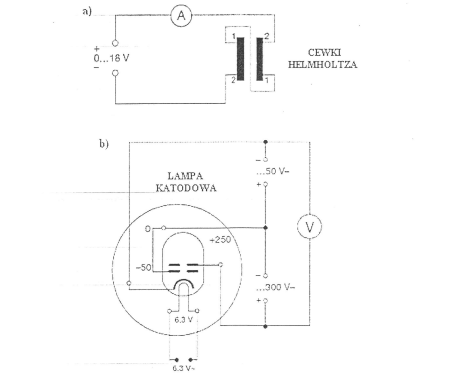
\includegraphics[scale=0.5]{cw45/schemat.png}
    \caption{Schemat wykorzystanego układu pomiarowego}
\end{figure}
\section{Wyniki Pomiarów}
Najpierw zespół ustalił napięcie siatkowe lampy $U_l$.
\begin{align*}
   U_l= 40 \si{V}
\end{align*}
Następnie  dla poszczególnych wartości napięcia anodowego zespół odczytał na amperomierzu takie natężenie i
prąd w cewkach, przy których kołowy tor wiazki elektronów w lampie trafia
na kolejne szczeble drabinki. Dla każdego szczebla wynik został zapisany trzykronie jako $I_1$, $I_2$ i $I_3$. Wyniki zapisano w tabeli \ref{tabel:1}
\begin{table}[H]
    \centering
    \begin{tabular}{|c|c|c|c|c|c|c|c|c|c|c|c|c|}
    \hline
        Promień r[cm] & \multicolumn{6}{c|}{2}  \multicolumn{3}{c|}{3} \multicolumn{3}{c|}{4} \multicolumn{3}{c|}{5}  \\ \hline
        Napięcie U[V]  $\downarrow$   & I_1 & I_2 & I_3 & I_1 & I_2 & I_3 & I_1 & I_2 & I_3 & I_1 & I_2 & I_3 \\ \hline
        125 & 3,15 & 3,18 & 3,18 & 1,97 & 1,98 & 1,97 & 1,44 & 1,44 & 1,43 & 1,15 & 1,14 & 1,16 \\ \hline
        150 & 3,38 & 3,37 & 3,38 & 2,16 & 2,15 & 2,15 & 1,56 & 1,56 & 1,56 & 1,24 & 1,24 & 1,24 \\ \hline
        175 & 3,62 & 3,61 & 3,6 & 2,33 & 2,33 & 2,34 & 1,7 & 1,7 & 1,7 & 1,34 & 1,34 & 1,35 \\ \hline
        200 & 3,83 & 3,84 & 3,84 & 2,59 & 2,5 & 2,5 & 1,82 & 1,82 & 1,82 & 1,44 & 1,44 & 1,44 \\ \hline
        225 & 4,02 & 4,05 & 4,04 & 2,64 & 2,63 & 2,63 & 1,93 & 1,93 & 1,93 & 1,53 & 1,53 & 1,52 \\ \hline
        250 & 4,21 & 4,23 & 4,21 & 2,76 & 2,76 & 2,76 & 2,03 & 2,03 & 2,03 & 1,6 & 1,61 & 1,6 \\ \hline
    \end{tabular}
    \caption{Wyniki pomiarów zmierzonego prądu dla sześciu róznych napięć anodowych}
    \label{tabel:1}
\end{table}

\section{Opracowanie wyników}
Wartość $\frac{e}{m}$ obliczamy dla każdego pomiaru $(U, I, r)$,
gdzie $I$ jest uśrednionym pomiarem natężenia prądu równym $\frac{I_1 + I_2 + I_3}{3}$,
podstawiając te wartości do \eqref{eq:em} razem z $n = 154$ i
promieniem cewki $R = 0.2$m. Wyniki obliczeń wraz z uśrednionymi $I$
zapisano w tabeli \ref{tab:2}.

\begin{table}[H]
\begin{tabular}{|l|llll|llll|llll|}
\hline
Napięcie{[}V{]}                                         & \multicolumn{4}{c|}{125}                                                                                          & \multicolumn{4}{c|}{150}                                                                                          & \multicolumn{4}{c|}{175}                                                                                          \\ \hline
r{[}cm{]}                                               & \multicolumn{1}{l|}{2}     & \multicolumn{1}{l|}{3}     & \multicolumn{1}{l|}{4}     & 5                          & \multicolumn{1}{l|}{2}     & \multicolumn{1}{l|}{3}     & \multicolumn{1}{l|}{4}     & 5                          & \multicolumn{1}{l|}{2}     & \multicolumn{1}{l|}{3}     & \multicolumn{1}{l|}{4}     & 5                          \\ \hline
Natężenie I{[}A{]}                                      & \multicolumn{1}{l|}{3,17}  & \multicolumn{1}{l|}{1,97}  & \multicolumn{1}{l|}{1,44}  & 1,15                       & \multicolumn{1}{l|}{3,38}  & \multicolumn{1}{l|}{2,15}  & \multicolumn{1}{l|}{1,56}  & 1,24                       & \multicolumn{1}{l|}{3,61}  & \multicolumn{1}{l|}{2,33}  & \multicolumn{1}{l|}{1,70}  & 1,34                       \\ \hline
e/m {[}10\textasciicircum{}9 V/A\textasciicircum{}2{]}  & \multicolumn{1}{c|}{130,1} & \multicolumn{1}{c|}{149,2} & \multicolumn{1}{c|}{158,3} & \multicolumn{1}{c|}{158,1} & \multicolumn{1}{c|}{137,6} & \multicolumn{1}{c|}{150,3} & \multicolumn{1}{c|}{161,1} & \multicolumn{1}{c|}{163,2} & \multicolumn{1}{c|}{140,4} & \multicolumn{1}{c|}{149,4} & \multicolumn{1}{c|}{158,3} & \multicolumn{1}{c|}{162,3} \\ \hline
Napięcie{[}V{]}                                         & \multicolumn{4}{c|}{200}                                                                                          & \multicolumn{4}{c|}{225}                                                                                          & \multicolumn{4}{c|}{250,00}                                                                                       \\ \hline
r{[}cm{]}                                               & \multicolumn{1}{l|}{2}     & \multicolumn{1}{l|}{3}     & \multicolumn{1}{l|}{4}     & 5                          & \multicolumn{1}{l|}{2}     & \multicolumn{1}{l|}{3}     & \multicolumn{1}{l|}{4}     & 5                          & \multicolumn{1}{l|}{2}     & \multicolumn{1}{l|}{3}     & \multicolumn{1}{l|}{4}     & 5                          \\ \hline
Natężenie I{[}A{]}                                      & \multicolumn{1}{l|}{3,84}  & \multicolumn{1}{l|}{2,53}  & \multicolumn{1}{l|}{1,82}  & 1,44                       & \multicolumn{1}{l|}{4,04}  & \multicolumn{1}{l|}{2,63}  & \multicolumn{1}{l|}{1,93}  & 1,53                       & \multicolumn{1}{l|}{4,22}  & \multicolumn{1}{l|}{2,76}  & \multicolumn{1}{l|}{2,03}  & 1,60                       \\ \hline
e/m  {[}10\textasciicircum{}9 V/A\textasciicircum{}2{]} & \multicolumn{1}{c|}{142,1} & \multicolumn{1}{c|}{145,2} & \multicolumn{1}{c|}{157,8} & \multicolumn{1}{c|}{161,4} & \multicolumn{1}{c|}{144,4} & \multicolumn{1}{c|}{150,8} & \multicolumn{1}{c|}{157,9} & \multicolumn{1}{c|}{161,5} & \multicolumn{1}{c|}{147,0} & \multicolumn{1}{c|}{152,5} & \multicolumn{1}{c|}{158,6} & \multicolumn{1}{c|}{162,7} \\ \hline
\end{tabular}
\caption{Wyniki $\frac{e}{m}$ dla każdego pomiaru $(U, I, r)$.}
\label{tab:2}
\end{table}
Dla uproszczenia zapisu przyjmiemy, że $k = \frac{e}{m}$.
Za uzyskaną z eksperymentu wartość $\frac{e}{m}$ przyjmiemy
średnią z uzyskanych wyników
\begin{align*}
    \frac{e}{m} = k = \bar{k} = \frac{1}{n}\sum k_i \approx \SI{152.5e9}{\emunit}
\end{align*}
Za niepewność otrzymanego wyniku przyjmiemy średni błąd kwadratowy
\begin{align*}
    u(k) = \frac{1}{n(n-1)}\sum(k_i - \bar{k}) \approx \SI{1.8e9}{\emunit}.
\end{align*}
W takim razie niepewność rozszerzona wynosi
\begin{align*}
    U(k) = 2u(k) = \SI{3.6e9}{\emunit}.
\end{align*}
Za wartość tablicową $\frac{e}{m}$ przyjmiemy wynik dzielenia
tablicowych wartości ładunku elektronu i jego masy
\begin{align*}
    k_{tab} = \frac{e_{tab}}{m_{tab}} = \frac{\SI{1.6e-19}{C}}{\SI{9.1e-31}{kg}} \approx \SI{175.8}{\emunit}.
\end{align*}
Z porównania tych wartości w granicach błędu rozszerzonego
\begin{align*}
    |k - k_{tab}| &= \SI{23.3e9}{\emunit}\\
    U(k) &= \SI{3.6e9}{\emunit}\\
    |k - k_{tab}| &> U(k)
\end{align*}
wynika, że otrzymany wynik nie zgadza się z odpowiadającą mu
wartością tablicową.
\section{Wnioski}
Metodą badania ruchu wiązki elektronów w jednorodnym polu
magnetycznym wytworzonym przez układ dwóch cewek Helmholtza
otrzymaliśmy wartość ładunku właściwego elektronu 
$\frac{e}{m} = \SI{152.5e9}{\emunit}$ o niepewności 
$u(\frac{e}{m}) = \SI{1.8e9}{\emunit}$. Otrzymany wynik nie jest
zgodny z wartością tablicową. Zespół doszedł do wniosku, że wynika
to z wadliwego układu mierzącego, w którym wyniki dla różnych
napięć $U$ i promieni $r$ bardzo mocno się różniły.

\end{document}